Listing \ref{lst:stx:expressions} specifies the syntax of all kinds of \emph{expressions} in CML.
It also lists them in their order of precedence.

Observe that the grammar in listing \ref{lst:stx:expressions} has left recursions
(and thus it is ambiguous).
However, ANTLR \cite{antlr} resolves the ambiguity
based on the order in which the \emph{expression} alternatives are listed,
and so the order in listing \ref{lst:stx:expressions} defines the precedence among the operators for CML.

Also, according to ANTLR,
and as required by CML,
all \emph{expressions} in the grammar are left-to-right associative,
except for the \emph{exponentiation expression},
which is right-to-left associative,
as defined by the \textbf{<assoc=right>} clause.

\begin{code}
\verbatimfont{\small}
\lstinputlisting[language=antlr]{grammar/Expressions.txt}
\caption{Expression Concrete Syntax}
\label{lst:stx:expressions}
\end{code}

Figure \ref{fig:meta:expression} presents the \emph{Expression} metaclass
in an EMOF \cite{mof} class diagram.
For each kind of \emph{expression} parsed by the compiler,
an instance of an \emph{Expression} subclass will be created,
and its properties will be assigned
according to parsed information:

\begin{itemize}

\item \emph{kind}:
a \emph{String} value matching the \emph{Expression} subclass;
for example, for the \emph{Literal} subclass, \textbf{kind = "literal"}.

\item \emph{type}:
a derived attribute that computes the \emph{Type} of the \emph{expression};
each \emph{Expression} subclass will do its own \emph{Type} computation
by providing its own definition for this derived attribute.

\end{itemize}

\begin{figure}
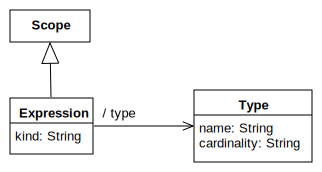
\includegraphics[width=\textwidth]{metamodel/expression}
\caption{Expression Abstract Syntax}
\label{fig:meta:expression}
\end{figure}
